






\chapter{Frames}
\label{sec:frames}

\section{The digital world ($\mathbb{Z}$)}

Pixels or voxels are defined over $\mathbb{Z}^2$ or $\mathbb{Z}^3$ and have integer coordinates. 


The voxel is a small rectangular cuboid that has a spatial extent. Our conventions are that the voxel coordinates design the center of the voxel. Let $(v_x, v_y, v_z)$ be the voxel size of image $I$, the spatial area of a voxel $M_{\mathbb{R}} = (x,y,z)$ in the real world $\mathbb{R}$ is the cuboid
$[x-v_x/2, x+v_x/2] \times [y-v_y/2, y+v_y/2] \times [z-v_z/2, z+v_z/2]$ (see figure \ref{fig:frame}). 


\begin{figure}[ht]
\begin{center}
 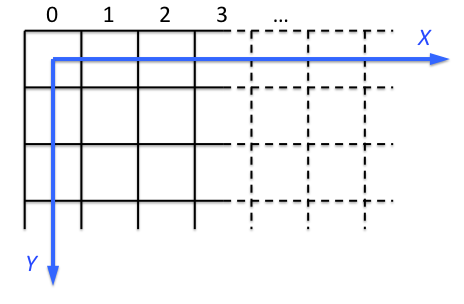
\includegraphics[height=5cm]{figures/fig-frame.png}
\end{center}
\caption{\label{fig:frame}Definition of the  field of view with respect to the  \textit{voxel} one. The origin of the \textit{real} frame is at the center of the upper left pixel/voxel, here the one of coordinate $(0,0,\ldots)$ (C/C++ conventions).}
\end{figure}

Let us consider an image that has a voxel size $v_x$ and a number of voxels of $d_x$ along the $X$ direction. From the C/C++ conventions, the $d_x$ voxels have coordinates in $\mathbb{Z}$ from $0$ to $d_x-1$. The length of the field of view (FOV) is obviously $v_x d_x$ and spans the interval $[v_x * 0 -v_x/2 , v_x*(d_x-1)+v_x/2]
= [-v_x/2, v_x d_x - v_x/2]$ in $\mathbb{R}$.

As a consequence, the center of the field of view in $\mathbb{Z}$ is (here in 3D)
\begin{displaymath}
C_{\mathbb{Z}} = 
\left(
\begin{array}{c}
\frac{(d_{x}-1)}{2} \\
\frac{(d_{y}-1)}{2} \\
\frac{(d_{z}-1)}{2}
\end{array}
\right)
\end{displaymath}

Converting voxel coordinates into real ones can trivially be done by multiplying by the voxel sizes (see section \ref{sec:frame:conversion}). The voxel with zero's coordinates defines then the origin of the \textit{real} frame.

\section{Image: $\mathbb{R} \leftrightarrow \mathbb{Z}$}
\label{sec:frame:conversion}


An image $I$ is defined over the discrete frame $\mathbb{Z}$ and a point $M$ may be defined either by its 'voxel' coordinates $(i,j,k)$, or by 'real' coordinates $(x,y,z)$ that can be deduced from $(i,j,k)$ thanks to the imaging acquisition information.

Conversion from the voxel frame, denoted $\mathbb{Z}$, to the real one, denoted $\mathbb{R}$, is achieved through conversion matrices that are associated with every image $I$.

Without any other specification, there are diagonal matrices with the voxel sizes (or their inverses) along the diagonal. Let $(v_x, v_y, v_z)$ be the voxel size of image $I$, thus a point $M_{\mathbb{R}} = (x,y,z)$ in the real frame $\mathbb{R}$ correspond to the voxel point $M_{\mathbb{Z}} = (i,j,k)$ in the voxel frame $\mathbb{Z}$ with
$$M_{\mathbb{R}} = \mathbf{H}_{I,\mathbb{R} \leftarrow \mathbb{Z}} M_{\mathbb{Z}}
\quad \mbox{ with } \quad
\mathbf{H}_{I,\mathbb{R} \leftarrow \mathbb{Z}} = \left( \begin{array}{cccc}
v_x & . & . & . \\
. & v_y & . & . \\
. & . & v_z & . \\
. & . & . & 1  
\end{array} \right)
$$
Accordingly,
$$M_{\mathbb{Z}} = \mathbf{H}_{I,\mathbb{Z} \leftarrow \mathbb{R}} M_{\mathbb{R}}
\quad \mbox{ with } \quad
\mathbf{H}_{I,\mathbb{Z} \leftarrow \mathbb{R}} = \left( \begin{array}{cccc}
1/v_x & . & . & . \\
. & 1/v_y & . & . \\
. & . & 1/v_z & . \\
. & . & . & 1  
\end{array} \right)
$$
Obviously, we have $\mathbf{H}_{I,\mathbb{Z} \leftarrow \mathbb{R}} = \mathbf{H}^{-1}_{I,\mathbb{R} \leftarrow \mathbb{Z}}$. Note that we use homogeneous coordinates (see section \ref{sec:homogeneous}) to define these matrices.


\begin{attention}
With such a default convention, the frame origins in both the real and the voxel frames superimpose. However, the frame origin in the real frame is not the upper left corner of the field of view (see figure \ref{fig:frame}).
\end{attention}

Note that the matrix $\mathbf{H}$ can be any linear matrix. E.g. they can be reorientation matrices that allows to map the voxel array in standard radiology conventions \footnote{Nifti and Inrimage image formats can embed such rigid transformations (the so-called qform matrices in Nifti format). However, such information can be lost when converting to other formats.}.






%%%%%%%%%%%%%%%%%%%%%%%%%%%%%%%%%%%%%%%
%
% transformations
%
%%%%%%%%%%%%%%%%%%%%%%%%%%%%%%%%%%%%%%%





\chapter{Transformations}


\section{Definitions}

\subsection{Linear transformations}

Classically, linear transformations (i.e. translations, rigid transformations, affine transformations, etc.) are expressed as combinations of a $3 \times 3$ matrix (representing the vectorial part of the transformation) $\mathbf{A}$ and a 3D vector $\mathbf{t}$ (representing the translation). Thus, the transformed point $M'$ of $M$ by the transformation $T=(\mathbf{A},\mathbf{t})$ is expressed by
\begin{displaymath}
M' = T(M) = \mathbf{A} M + \mathbf{t}
\end{displaymath}

Note that linear transformations are mainly expressed in homogeneous coordinates all along this document (see section \ref{sec:homogeneous:linear}), thus we will use the somewhat abusive notation
\begin{displaymath}
M' = \mathbf{T} M 
\end{displaymath}
where $\mathbf{T}$ is a $4 \times 4$ matrix.

\subsection{Vector fields}

Vector fields are used to encode non-linear transformations. For a transformation $T$, the vector $\mathbf{v}(M)$ at point $M$ is the displacement of the point $M$, meaning that 
\begin{displaymath}
M' = T(M) = M + \mathbf{v}(M)
\end{displaymath}







\section{Homogeneous coordinates}
\label{sec:homogeneous}

4D homogeneous coordinates are implicitly used. However, there are some  with transformations expressed as vector fields. 

\subsection{Linear transformations}
\label{sec:homogeneous:linear}

It is more convenient to express the linear transformations as $4 \times 4$ matrices embedding the translation, so combinations of linear transformations can be expressed by multiplications of matrices. Such a $4 \times 4$ matrix $\mathbf{T}$ is designed by
\begin{displaymath}
\mathbf{T} =
\left(
\begin{array}{ccc|c}
& & & \\
& \mathbf{A} & & \mathbf{t} \\
& & & \\ \hline
0 & 0 & 0 & 1
\end{array}
\right)
\end{displaymath}

A point $M$ has then implicitly 4 coordinates, the first three ones being the spatial coordinates $(x,y,z)$ and the last one being 1. We have thus 
\begin{displaymath}
M'
= T(M)
=
\left(
\begin{array}{l}
x' \\ y' \\ z' \\ 1
\end{array}
\right)
= \mathbf{T} M
= 
\left(
\begin{array}{ccc|c}
& & & \\
& \mathbf{A} & & \mathbf{t} \\
& & & \\ \hline
0 & 0 & 0 & 1
\end{array}
\right)
\left(
\begin{array}{l}
x \\ y \\ z \\ 1
\end{array}
\right)
\end{displaymath}


\subsection{Vector fields}

The transformation with a vector field is encoded by 
\begin{displaymath}
M' = M + \mathbf{v}(M)
\end{displaymath}
When composing (at left) with a linear transformation, we have
\begin{eqnarray}
M'' & = & \mathbf{A} M' + \mathbf{t} \nonumber \\
& = & \mathbf{A} M + \mathbf{A} \mathbf{v}(M) + \mathbf{t}
\label{eq:composition:linear:vector}
\end{eqnarray}

If homogeneous coordinates are used, it comes
\begin{eqnarray*}
M'' & = & \mathbf{T} M' 
\left( = \mathbf{A} M' + \mathbf{t} \right) \\
& = & \mathbf{T} M + \mathbf{T} \mathbf{v}(M) 
\end{eqnarray*}
From equation \ref{eq:composition:linear:vector}, it comes that 
\begin{displaymath}
\mathbf{T} \mathbf{v}(M) = \mathbf{A} \mathbf{v}(M)
\end{displaymath}
This is compatible with homogeneous coordinates if the fourth coordinate of $\mathbf{v}$ is $0$, indeed
\begin{displaymath}
\mathbf{T} \mathbf{v}
= 
\left(
\begin{array}{ccc|c}
& & & \\
& \mathbf{A} & & \mathbf{t} \\
& & & \\ \hline
0 & 0 & 0 & 1
\end{array}
\right)
\left(
\begin{array}{c}
\mathbf{v}_x \\ \mathbf{v}_y \\ \mathbf{v}_z \\ 0
\end{array}
\right)
= 
\left(
\begin{array}{c}
\mathbf{A} \mathbf{v} \\ \hline
0
\end{array}
\right)
\end{displaymath}













\section{'voxel' versus 'real' definitions}

%definitions for discrete images; $\mathbb{R} \leftrightarrow \mathbb{Z}$ conversion}

Recall that an image $I$ is defined over the discrete frame $\mathbb{Z}$. Thus a point $M$ of $I$ can be expressed either in the discrete frame in voxel coordinates (and will be denoted $M_{\mathbb{Z}}$) or in real coordinates (and will be denoted $M_{\mathbb{R}}$). Conversion matrices (see section \ref{sec:frame:conversion}) allow to go from the voxel frame to the real one, and conversely.

A transformation $T_{flo \leftarrow ref}$ from an image $I_{ref}$ towards an image $I_{flo}$ can be then either defined in the voxel frame or in the real one. These transformations are denoted respectively $T_{flo \leftarrow ref,\mathbb{Z}}$ and $T_{flo \leftarrow ref,\mathbb{R}}$:
\begin{displaymath}
\begin{array}{ll}
T_{flo \leftarrow ref,\mathbb{Z}}: &
I_{ref} \rightarrow I_{flo}\\
& M_{ref,\mathbb{Z}} \mapsto M_{flo,\mathbb{Z}}
\end{array}
\end{displaymath}
and
\begin{displaymath}
\begin{array}{ll}
T_{flo \leftarrow ref,\mathbb{R}}: &
I_{ref} \rightarrow I_{flo}\\
& M_{ref,\mathbb{R}} \mapsto M_{flo,\mathbb{R}}
\end{array}
\end{displaymath}

We have then 
\begin{eqnarray*}
M_{flo,\mathbb{Z}} & = & 
T_{flo \leftarrow ref,\mathbb{Z}}(M_{ref,\mathbb{Z}}) \\
M_{flo,\mathbb{R}} & = & 
T_{flo \leftarrow ref,\mathbb{R}}(M_{ref,\mathbb{R}})
\end{eqnarray*}

Transformations in 'voxel' coordinates are required for image resampling, while transformations in 'real' coordinates may be necessary when dealing when some transformation classes (e.g. rigid) or to compute some measurements (e.g. mean displacements) in world units. Thus, conversion of these transformations from the voxel world to the real one, using the image conversion matrices (see section \ref{sec:frame:conversion}), has to be made explicit.

\subsection{Linear transformations}

Linear transformations can be expressed by $4x4$ matrices in homogeneous coordinates (see section \ref{sec:homogeneous:linear}), thus we have 
\begin{eqnarray*}
M_{flo,\mathbb{Z}} & = & 
T_{flo \leftarrow ref,\mathbb{Z}} M_{ref,\mathbb{Z}}  \\
M_{flo,\mathbb{R}} & = & 
T_{flo \leftarrow ref,\mathbb{R}} M_{ref,\mathbb{R}}
\end{eqnarray*}

To convert the transformations from the voxel world to the real one (and conversely), we apply the composition rules that are here simply matrices multiplication:
$$
\mathbf{T}_{flo \leftarrow ref, \mathbb{Z}} 
=
\mathbf{H}_{flo,\mathbb{Z} \leftarrow \mathbb{R}} \circ
\mathbf{T}_{flo \leftarrow ref, \mathbb{R}} \circ
\mathbf{H}_{ref,\mathbb{R} \leftarrow \mathbb{Z}}
$$
and
$$
\mathbf{T}_{flo \leftarrow ref, \mathbb{R}} 
=
\mathbf{H}_{flo,\mathbb{R} \leftarrow \mathbb{Z}} \circ
\mathbf{T}_{flo \leftarrow ref, \mathbb{Z}} \circ
\mathbf{H}_{ref,\mathbb{Z} \leftarrow \mathbb{R}}
$$


\subsection{Vector fields}

The difficulty comes from the fact that the non-linear transformation is encoded by a displacement/vector field that is defined over a discrete lattice (i.e. an image). We have then
\begin{eqnarray*}
M_{flo,\mathbb{Z}} & = & 
T_{flo \leftarrow ref,\mathbb{Z}}(M_{ref,\mathbb{Z}}) \\
& = &
M_{ref,\mathbb{Z}} + 
\mathbf{v}_{flo \leftarrow ref, \mathbb{Z}}(M_{ref, \mathbb{Z}}) \\
M_{flo,\mathbb{R}} & = & 
T_{flo \leftarrow ref,\mathbb{R}}(M_{ref,\mathbb{R}}) \\
& = &
M_{ref,\mathbb{R}} + 
\mathbf{v}_{flo \leftarrow ref, \mathbb{R}}(M_{ref, \mathbb{Z}}) \\
& = &
M_{ref,\mathbb{R}} + 
\mathbf{v}_{flo \leftarrow ref, \mathbb{R}}(\mathbf{H}_{ref, \mathbb{Z} \leftarrow \mathbb{R}}  M_{ref, \mathbb{R}})
\end{eqnarray*}
where $\mathbf{H}_{ref, \mathbb{Z} \leftarrow \mathbb{R}}$ denotes the conversion matrix from the real world $\mathbb{R}$ to the discrete world $\mathbb{Z}$ for image $I_{ref}$.

The vector field $\mathbf{v}$ indicates the displacement at every point. For a transformation from image $I_{ref}$ to image $I_{flo}$, this vector is defined on the same frame than $I_{ref}$. Thus the vector in \textit{real} coordinates $\mathbf{v}_{flo \leftarrow ref, \mathbb{R}}$ at $M_{\mathbb{R}}$ gives the displacement of the point $M_{\mathbb{R}}$.

However, since $\mathbf{v}_{flo \leftarrow ref}$ is defined over a discrete lattice, the vector image stores the vectors $\mathbf{v}_{\mathbb{R}}(M_{\mathbb{Z}})$, thus $\mathbf{v}_{\mathbb{R}}$ at $M_{\mathbb{R}}$ is $\mathbf{v}_{\mathbb{R}}( \mathbf{H}_{\mathbb{Z} \leftarrow \mathbb{R}} M_{\mathbb{R}} )$.


\subsubsection{Vector fields: $\mathbb{R} \rightarrow \mathbb{Z}$}




The transformation $\mathbf{T}_{flo \leftarrow ref, \mathbb{R}}$ from image $I_{ref}$ to image $I_{flo}$ is defined by the vector field $\mathbf{v}_{flo \leftarrow ref,\mathbb{R}}$
\begin{eqnarray*}
M_{flo,\mathbb{R}} & = & 
\mathbf{T}(M_{ref,\mathbb{R}}) = M_{ref,\mathbb{R}} + \mathbf{v}_{flo \leftarrow ref,\mathbb{R}}( \mathbf{H}_{ref, \mathbb{Z} \leftarrow \mathbb{R}} M_{ref,\mathbb{R}} )\\
& = & 
\mathbf{T}(M_{ref,\mathbb{R}}) = M_{ref,\mathbb{R}} + \mathbf{v}_{flo \leftarrow ref,\mathbb{R}}(M_{ref,\mathbb{Z}} )
\end{eqnarray*}

When expressing this formula in the discrete lattice, it comes
\begin{displaymath}
\mathbf{H}_{flo, \mathbb{R} \leftarrow \mathbb{Z}} M_{flo,\mathbb{Z}}
=
\mathbf{H}_{ref, \mathbb{R} \leftarrow \mathbb{Z}} M_{ref,\mathbb{Z}}
+ \mathbf{v}_{flo \leftarrow ref,\mathbb{R}}( M_{ref,\mathbb{Z}} )
\end{displaymath}
\begin{displaymath}
M_{flo,\mathbb{Z}} 
=
\mathbf{H}^{-1}_{flo, \mathbb{R} \leftarrow \mathbb{Z}}
\circ \mathbf{H}_{ref, \mathbb{R} \leftarrow \mathbb{Z}} 
M_{ref,\mathbb{Z}}
+ \mathbf{H}^{-1}_{flo, \mathbb{R} \leftarrow \mathbb{Z}}
\circ \mathbf{v}_{flo \leftarrow ref,\mathbb{R}}( M_{ref,\mathbb{Z}} )
\end{displaymath}


The displacement in \textit{voxel} coordinates $\mathbf{v}_{flo \leftarrow ref,\mathbb{Z}}$ (associated to $\mathbf{T}_{flo \leftarrow ref,\mathbb{Z}}$) is then defined by
\begin{eqnarray*}
\lefteqn{\mathbf{v}_{flo \leftarrow ref,\mathbb{Z}}( M_{ref,\mathbb{Z}} )
 =  M_{flo,\mathbb{Z}} - M_{ref,\mathbb{Z}}} \\
& = & 
\left( \mathbf{H}^{-1}_{flo, \mathbb{R} \leftarrow \mathbb{Z}}
 \circ \mathbf{H}_{ref, \mathbb{R} \leftarrow \mathbb{Z}} - \mathbf{Id} \right)
 M_{ref,\mathbb{Z}}
 + \mathbf{H}^{-1}_{flo, \mathbb{R} \leftarrow \mathbb{Z}}
 \circ \mathbf{v}_{flo \leftarrow ref,\mathbb{R}}( M_{ref,\mathbb{Z}} ) \\
 & = & 
\left( \mathbf{H}_{flo, \mathbb{Z} \leftarrow \mathbb{R}}
 \circ \mathbf{H}_{ref, \mathbb{R} \leftarrow \mathbb{Z}} - \mathbf{Id} \right)
 M_{ref,\mathbb{Z}}
 + \mathbf{H}_{flo, \mathbb{Z} \leftarrow \mathbb{R}}
 \circ \mathbf{v}_{flo \leftarrow ref,\mathbb{R}}( M_{ref,\mathbb{Z}} ) \\
\end{eqnarray*}
(where $\mathbf{Id}$ denotes the identity matrix) and may be different from a simple scaling of the vector field defined in \textit{real} coordinates.

\subsubsection{Vector fields: $\mathbb{Z} \rightarrow \mathbb{R}$}

We have 
\begin{displaymath}
M_{flo,\mathbb{Z}} = M_{ref,\mathbb{Z}} 
+ \mathbf{v}_{flo \leftarrow ref,\mathbb{Z}}( M_{ref,\mathbb{Z}} )
\end{displaymath}

When expressing this formula in the real world, it comes
\begin{displaymath}
\mathbf{H}_{flo, \mathbb{Z} \leftarrow \mathbb{R}} 
M_{flo,\mathbb{R}}
=
\mathbf{H}_{ref, \mathbb{Z} \leftarrow \mathbb{R}} 
M_{ref,\mathbb{R}}
+ \mathbf{v}_{flo \leftarrow ref,\mathbb{Z}}( M_{ref,\mathbb{Z}} ) \\
\end{displaymath}
\begin{displaymath}
M_{flo,\mathbb{R}}
=
\mathbf{H}^{-1}_{flo, \mathbb{Z} \leftarrow \mathbb{R}}
\circ 
\mathbf{H}_{ref, \mathbb{Z} \leftarrow \mathbb{R}}
M_{ref,\mathbb{R}}
+ 
\mathbf{H}^{-1}_{flo, \mathbb{Z} \leftarrow \mathbb{R}}
\circ \mathbf{v}_{flo \leftarrow ref,\mathbb{Z}}( M_{ref,\mathbb{Z}} )
\end{displaymath}

The displacement in \textit{real} coordinates $\mathbf{v}_{flo \leftarrow ref,\mathbb{R}}$ is then defined by
\begin{eqnarray*}
\lefteqn{
\mathbf{v}_{flo \leftarrow ref,\mathbb{R}}( M_{ref,\mathbb{Z}} )
= M_{flo,\mathbb{R}} - M_{ref,\mathbb{R}}} \\
& = & 
\left(
\mathbf{H}^{-1}_{flo, \mathbb{Z} \leftarrow \mathbb{R}}
\circ 
\mathbf{H}_{ref, \mathbb{Z} \leftarrow \mathbb{R}}
- \mathbf{Id} \right) M_{ref,\mathbb{R}}
+ 
\mathbf{H}^{-1}_{flo, \mathbb{Z} \leftarrow \mathbb{R}}
\circ \mathbf{v}_{flo \leftarrow ref,\mathbb{Z}}( M_{ref,\mathbb{Z}} ) \\
& = & 
\left(
\mathbf{H}^{-1}_{flo, \mathbb{Z} \leftarrow \mathbb{R}}
\circ 
\mathbf{H}_{ref, \mathbb{Z} \leftarrow \mathbb{R}}
- \mathbf{Id} \right) 
\mathbf{H}_{ref, \mathbb{R} \leftarrow \mathbb{Z}}
M_{ref,\mathbb{Z}}
+ 
\mathbf{H}_{flo, \mathbb{R} \leftarrow \mathbb{Z}}
\circ \mathbf{v}_{flo \leftarrow ref,\mathbb{Z}}( M_{ref,\mathbb{Z}} ) \\
& = & 
\left(
\mathbf{H}_{flo, \mathbb{R} \leftarrow \mathbb{Z}}
-
\mathbf{H}_{ref, \mathbb{R} \leftarrow \mathbb{Z}}
\right)
M_{ref,\mathbb{Z}}
+ 
\mathbf{H}_{flo, \mathbb{R} \leftarrow \mathbb{Z}}
\circ \mathbf{v}_{flo \leftarrow ref,\mathbb{Z}}( M_{ref,\mathbb{Z}} ) \\
\end{eqnarray*}





\section{Transformations: linear $\rightarrow$ vector field}

$\mathbf{T}_{flo \leftarrow ref, \mathbb{R}}$ is a linear transformation in real space. We have then
\begin{displaymath}
M_{flo, \mathbb{R}} = 
\mathbf{T}_{flo \leftarrow ref, \mathbb{R}}
M_{ref, \mathbb{R}}
\end{displaymath}
For vector fields, the transformation is expressed by
\begin{displaymath}
M_{flo, \mathbb{R}} = 
M_{ref, \mathbb{R}} 
+ \mathbf{v}_{flo \leftarrow ref, \mathbb{R}}(M_{ref, \mathbb{Z}})
\end{displaymath}
We have then
\begin{eqnarray*}
\mathbf{v}_{flo \leftarrow ref, \mathbb{R}}(M_{ref, \mathbb{Z}}) & = & 
M_{flo, \mathbb{R}} - M_{ref, \mathbb{R}} \\
& = &
\mathbf{T}_{flo \leftarrow ref, \mathbb{R}}
M_{ref, \mathbb{R}} - M_{ref, \mathbb{R}} \\
& = &
\left( \mathbf{T}_{flo \leftarrow ref, \mathbb{R}} - \mathbf{Id} \right) \circ
\mathbf{H}_{ref, \mathbb{R} \leftarrow \mathbb{Z}} M_{ref, \mathbb{Z}} \\
& = &
\left( \mathbf{H}_{flo,\mathbb{R} \leftarrow \mathbb{Z}} \circ
\mathbf{T}_{flo \leftarrow ref, \mathbb{Z}} \circ
\mathbf{H}_{ref,\mathbb{Z} \leftarrow \mathbb{R}} - \mathbf{Id} \right) \circ
\mathbf{H}_{ref, \mathbb{R} \leftarrow \mathbb{Z}} M_{ref, \mathbb{Z}} \\
\end{eqnarray*}

Remarks:
\begin{itemize}

\item Estimating the vector field in real/world units $\mathbf{v}_{flo \leftarrow ref, \mathbb{R}}$ from a linear transformation in real/world units $\mathbf{T}_{flo \leftarrow ref, \mathbb{Z}}$ is done with 
\begin{displaymath}
\left( \mathbf{T}_{flo \leftarrow ref, \mathbb{R}} - \mathbf{Id} \right) \circ
\mathbf{H}_{ref, \mathbb{R} \leftarrow \mathbb{Z}} M_{ref, \mathbb{Z}}
\end{displaymath}
Note that the voxel-to-world transformation for the reference image/frame $\mathbf{H}_{ref, \mathbb{R} \leftarrow \mathbb{Z}}$ is also embedded in the non-linear transformation $\mathbf{v}_{flo \leftarrow ref, \mathbb{R}}$.

\item Estimating the vector field in real/world units $\mathbf{v}_{flo \leftarrow ref, \mathbb{R}}$ from a linear transformation in voxel units $\mathbf{T}_{flo \leftarrow ref, \mathbb{Z}}$ 
\begin{eqnarray*}
\lefteqn{\mathbf{v}_{flo \leftarrow ref, \mathbb{R}}(M_{ref, \mathbb{Z}}) = } \\
& &
\left( \mathbf{H}_{flo,\mathbb{R} \leftarrow \mathbb{Z}} \circ
\mathbf{T}_{flo \leftarrow ref, \mathbb{Z}} \circ
\mathbf{H}_{ref,\mathbb{Z} \leftarrow \mathbb{R}} - \mathbf{Id} \right) \circ
\mathbf{H}_{ref, \mathbb{R} \leftarrow \mathbb{Z}} M_{ref, \mathbb{Z}}
\end{eqnarray*}
requires to have the voxel-to-world transformation for the floating image/frame $\mathbf{H}_{flo,\mathbb{R} \leftarrow \mathbb{Z}}$ at hand.

\item When $\mathbf{T}_{flo \leftarrow ref, \mathbb{R}}$ is a pure translation $\mathbf{t}_{\mathbb{R}}$, meaning that 
$M_{flo, \mathbb{R}} = 
\mathbf{Id} M_{ref, \mathbb{R}} + \mathbf{t}_{\mathbb{R}}$, we have then
\begin{displaymath}
\mathbf{v}_{flo \leftarrow ref, \mathbb{R}}(M_{ref, \mathbb{Z}}) = \mathbf{t}_{\mathbb{R}}
\end{displaymath}

\end{itemize}










\section{Transformation composition}

We simply use the composition rules to  transformation composition.
\begin{displaymath}
\mathbf{T}_{K \leftarrow I, \mathbb{R}}
= 
\mathbf{T}_{K \leftarrow J, \mathbb{R}}
\circ
\mathbf{T}_{J \leftarrow I, \mathbb{R}}
\end{displaymath}
and
\begin{displaymath}
\mathbf{T}_{K \leftarrow I, \mathbb{Z}}
= 
\mathbf{T}_{K \leftarrow J, \mathbb{Z}}
\circ
\mathbf{T}_{J \leftarrow I, \mathbb{Z}}
\end{displaymath}



\subsection{Linear $\circ$ linear}

The composition is quite trivial, since it only uses matrices multiplication.



\subsection{Linear $\circ$ vector field in $\mathbb{R}$ }

\begin{eqnarray*}
M_{J, \mathbb{R}} & = &
M_{I, \mathbb{R}} 
+ \mathbf{v}_{J \leftarrow I, \mathbb{R}}
(\mathbf{H}_{I, \mathbb{Z} \leftarrow \mathbb{R}}  M_{I, \mathbb{R}}) \\
& = & 
\mathbf{H}_{I, \mathbb{R} \leftarrow \mathbb{Z}} M_{I, \mathbb{Z}}
+ \mathbf{v}_{J \leftarrow I, \mathbb{R}}(M_{I, \mathbb{Z}}) \\
M_{K, \mathbb{R}} & = &
 \mathbf{T}_{K \leftarrow J, \mathbb{R}} M_{J, \mathbb{R}} \\
& = &
\mathbf{T}_{K \leftarrow J, \mathbb{R}} 
\mathbf{H}_{I, \mathbb{R} \leftarrow \mathbb{Z}} 
M_{I, \mathbb{Z}} 
+ \mathbf{T}_{K \leftarrow J, \mathbb{R}} 
\mathbf{v}_{J \leftarrow I, \mathbb{R}}(M_{I, \mathbb{Z}})
\end{eqnarray*}

\begin{eqnarray*}
\mathbf{v}_{K \leftarrow I, \mathbb{R}}(M_{I, \mathbb{Z}})
& = &
M_{K, \mathbb{R}} - M_{I, \mathbb{R}} \\
& = &
\left( \mathbf{T}_{K \leftarrow J, \mathbb{R}} - \mathbf{Id} \right)
\circ 
\mathbf{H}_{I, \mathbb{R} \leftarrow \mathbb{Z}} 
M_{I, \mathbb{Z}} 
+ \mathbf{T}_{K \leftarrow J, \mathbb{R}} 
\mathbf{v}_{J \leftarrow I, \mathbb{R}}(M_{I, \mathbb{Z}})
\end{eqnarray*}



\subsection{Linear $\circ$ vector field in $\mathbb{Z}$ }

\begin{eqnarray*}
M_{J, \mathbb{Z}} & = &
M_{I, \mathbb{Z}} 
+ \mathbf{v}_{J \leftarrow I, \mathbb{Z}}(M_{I, \mathbb{Z}}) \\
M_{K, \mathbb{Z}} & = &
 \mathbf{T}_{K \leftarrow J, \mathbb{Z}} M_{J, \mathbb{Z}} \\
& = &
\mathbf{T}_{K \leftarrow J, \mathbb{Z}} 
M_{I, \mathbb{Z}} 
+ \mathbf{T}_{K \leftarrow J, \mathbb{Z}} 
\mathbf{v}_{J \leftarrow I, \mathbb{Z}}(M_{I, \mathbb{Z}})
\end{eqnarray*}

\begin{eqnarray*}
\mathbf{v}_{K \leftarrow I, \mathbb{Z}}(M_{I, \mathbb{Z}})
& = &
M_{K, \mathbb{Z}} - M_{I, \mathbb{Z}} \\
& = &
\left( \mathbf{T}_{K \leftarrow J, \mathbb{Z}} - \mathbf{Id} \right)
M_{I, \mathbb{Z}} 
+ \mathbf{T}_{K \leftarrow J, \mathbb{Z}} 
\mathbf{v}_{J \leftarrow I, \mathbb{Z}}(M_{I, \mathbb{Z}})
\end{eqnarray*}





\subsection{Vector field $\circ$ linear in $\mathbb{R}$ }

\begin{eqnarray*}
M_{J, \mathbb{R}} & = &  
\mathbf{T}_{J \leftarrow I, \mathbb{R}} M_{I, \mathbb{R}}  \\
M_{K, \mathbb{R}} & = &
M_{J, \mathbb{R}} 
+ \mathbf{v}_{K \leftarrow J, \mathbb{R}}(\mathbf{H}_{J, \mathbb{Z} \leftarrow \mathbb{R}}  M_{J, \mathbb{R}}) \\
& = &
\mathbf{T}_{J \leftarrow I, \mathbb{R}} M_{I, \mathbb{R}}
+ \mathbf{v}_{K \leftarrow J, \mathbb{R}}(\mathbf{H}_{J, \mathbb{Z} \leftarrow \mathbb{R}}  \mathbf{T}_{J \leftarrow I, \mathbb{R}} M_{I, \mathbb{R}} )
\end{eqnarray*}

\begin{eqnarray*}
\mathbf{v}_{K \leftarrow I, \mathbb{R}}(M_{I, \mathbb{Z}})
& = &
M_{K, \mathbb{R}} - M_{I, \mathbb{R}} \\
& = &
\left( \mathbf{T}_{J \leftarrow I, \mathbb{R}} - \mathbf{Id} \right)
\circ 
\mathbf{H}_{I, \mathbb{R} \leftarrow \mathbb{Z}} 
M_{I, \mathbb{Z}}  \\
& & {}
+ 
\mathbf{v}_{K \leftarrow J, \mathbb{R}}
(\mathbf{H}_{J, \mathbb{Z} \leftarrow \mathbb{R}}
\mathbf{T}_{J \leftarrow I, \mathbb{R}} 
\mathbf{H}_{I, \mathbb{R} \leftarrow \mathbb{Z}}
M_{I, \mathbb{Z}} )
\end{eqnarray*}



\subsection{Vector field $\circ$ linear in $\mathbb{Z}$ }

\begin{eqnarray*}
M_{J, \mathbb{Z}} &  =  &
\mathbf{T}_{J \leftarrow I, \mathbb{Z}} M_{I, \mathbb{Z}} \\
M_{K, \mathbb{Z}} & = &
M_{J, \mathbb{Z}} 
+ \mathbf{v}_{K \leftarrow J, \mathbb{Z}}(M_{J, \mathbb{Z}}) \\
& = &
\mathbf{T}_{J \leftarrow I, \mathbb{Z}} M_{I, \mathbb{Z}} 
+ \mathbf{v}_{K \leftarrow J, \mathbb{Z}}(\mathbf{T}_{J \leftarrow I, \mathbb{Z}} M_{I, \mathbb{Z}} )
\end{eqnarray*}

\begin{eqnarray*}
\mathbf{v}_{K \leftarrow I, \mathbb{Z}}(M_{I, \mathbb{Z}})
& = &
M_{K, \mathbb{Z}} - M_{I, \mathbb{Z}} \\
& = &
\left( \mathbf{T}_{J \leftarrow I, \mathbb{Z}} - \mathbf{Id} \right)
M_{I, \mathbb{Z}}
+ \mathbf{v}_{K \leftarrow J, \mathbb{Z}}
( \mathbf{T}_{J \leftarrow I, \mathbb{Z}} M_{I, \mathbb{Z}} )
\end{eqnarray*}


\subsection{Vector field $\circ$ vector field in $\mathbb{R}$ }

\begin{eqnarray*}
M_{J, \mathbb{R}} & =  &
M_{I, \mathbb{R}} 
+ \mathbf{v}_{J \leftarrow I, \mathbb{R}}(\mathbf{H}_{I, \mathbb{Z} \leftarrow \mathbb{R}}  M_{I, \mathbb{R}}) \\
& = &
\mathbf{H}_{I, \mathbb{R} \leftarrow \mathbb{Z}} M_{I, \mathbb{Z}}
+ \mathbf{v}_{J \leftarrow I, \mathbb{R}}(M_{I, \mathbb{Z}}) \\
M_{K, \mathbb{R}} & = &
M_{J, \mathbb{R}} 
+ \mathbf{v}_{K \leftarrow J, \mathbb{R}}(\mathbf{H}_{J, \mathbb{Z} \leftarrow \mathbb{R}}  M_{J, \mathbb{R}}) \\
& = &
M_{I, \mathbb{R}}
+ \mathbf{v}_{J \leftarrow I, \mathbb{R}}(M_{I, \mathbb{Z}}) \\
& & {}
+ \mathbf{v}_{K\leftarrow J, \mathbb{R}}\left(
\mathbf{H}_{J, \mathbb{Z} \leftarrow \mathbb{R}} 
\left( 
\mathbf{H}_{I, \mathbb{R} \leftarrow \mathbb{Z}} M_{I, \mathbb{Z}}
+ 
\mathbf{v}_{J \leftarrow I, \mathbb{R}}(M_{I, \mathbb{Z}}
\right)
\right)
\end{eqnarray*}


\begin{eqnarray*}
\mathbf{v}_{K \leftarrow I, \mathbb{R}}(M_{I, \mathbb{Z}})
& = &
M_{K, \mathbb{R}} - M_{I, \mathbb{R}} \\
& = &
\mathbf{v}_{J \leftarrow I, \mathbb{R}}(M_{I, \mathbb{Z}}) \\
& & {}
+ \mathbf{v}_{K \leftarrow J, \mathbb{R}}
\left(
\mathbf{H}_{J, \mathbb{Z} \leftarrow \mathbb{R}} 
\left( 
\mathbf{H}_{I, \mathbb{R} \leftarrow \mathbb{Z}} M_{I, \mathbb{Z}}
+ 
\mathbf{v}_{J \leftarrow I, \mathbb{R}}(M_{I, \mathbb{Z}}
\right)
\right) \\
& = &
\mathbf{v}_{J \leftarrow I, \mathbb{R}}(M_{I, \mathbb{Z}}) \\
& & {}
+ \mathbf{v}_{K \leftarrow J, \mathbb{R}}
\left(
\mathbf{H}_{J, \mathbb{Z} \leftarrow \mathbb{R}} 
\circ
\mathbf{H}_{I, \mathbb{R} \leftarrow \mathbb{Z}} M_{I, \mathbb{Z}}
+ 
\mathbf{H}_{J, \mathbb{Z} \leftarrow \mathbb{R}} 
\circ \mathbf{v}_{J \leftarrow I, \mathbb{R}}(M_{I, \mathbb{Z}})
\right)
\end{eqnarray*}





\subsection{Vector field $\circ$ vector field in $\mathbb{Z}$ }


\begin{eqnarray*}
M_{J, \mathbb{Z}} & =  &
M_{I, \mathbb{Z}} 
+ \mathbf{v}_{J \leftarrow I, \mathbb{Z}}( M_{I, \mathbb{Z}}) \\
M_{K, \mathbb{Z}} & = &
M_{J, \mathbb{Z}} 
+ \mathbf{v}_{K \leftarrow J, \mathbb{Z}}(M_{J, \mathbb{Z}}) \\
& = &
M_{I, \mathbb{Z}}
+ \mathbf{v}_{J \leftarrow I, \mathbb{Z}}(M_{I, \mathbb{Z}}) 
+ \mathbf{v}_{K\leftarrow J, \mathbb{Z}}\left(
M_{I, \mathbb{Z}} 
+ \mathbf{v}_{J \leftarrow I, \mathbb{Z}}( M_{I, \mathbb{Z}})
\right)
\end{eqnarray*}


\begin{eqnarray*}
\mathbf{v}_{K \leftarrow I, \mathbb{Z}}(M_{I, \mathbb{Z}})
& = &
M_{K, \mathbb{Z}} - M_{I, \mathbb{Z}} \\
& = &
\mathbf{v}_{J \leftarrow I, \mathbb{Z}}(M_{I, \mathbb{Z}}) 
+ \mathbf{v}_{K\leftarrow J, \mathbb{Z}}\left(
M_{I, \mathbb{Z}} 
+ \mathbf{v}_{J \leftarrow I, \mathbb{Z}}( M_{I, \mathbb{Z}})
\right)
\end{eqnarray*}






\section{Field of view center alignment}
\label{sec:field:view:center:alignment}


For computational reasons, it may be useful to change the resolution of an image, typically dividing the dimensions by a factor 2 (and then multiplying the voxel sizes by 2). It allows to deal with smaller images while letting the FOV sizes unchanged.

However, because of our conventions where the frame origin is not at the upper left corner of the FOV but at the center of the upper left voxel, the transformation that goes from one frame to the other is a translation (the translation between the two origins).

Let us consider the general case where we want to build the translation that superimposes the FOV centers of two images $I_{ref}$ and $I_{flo}$. Without loss of generality, we only consider the $X$ direction. $I_{ref}$ and $I_{flo}$ have respectively a number of voxels of $d_{ref,x}$ and $d_{flo,x}$. The FOV intervals (in voxels) are respectively 
$[-1/2, d_{ref,x} - 1/2]$ and
$[-1/2, d_{flo,x} - 1/2]$ in $\mathbb{Z}$. The FOV centers along the $X$ direction are then respectively $\frac{(d_{ref,x}-1)}{2}$ and $\frac{(d_{fflo,x}-1)}{2}$. 

In 3D, the FOV centers of $I_{ref}$ and $I_{flo}$ are respectively
\begin{displaymath}
C_{ref,\mathbb{Z}} = 
\left(
\begin{array}{c}
\frac{(d_{r,x}-1)}{2} \\
\frac{(d_{r,y}-1)}{2} \\
\frac{(d_{r,z}-1)}{2}
\end{array}
\right)
\quad \textrm{ and } \quad
C_{flo,\mathbb{Z}} = 
\left(
\begin{array}{c}
\frac{(d_{f,x}-1)}{2} \\
\frac{(d_{f,y}-1)}{2} \\
\frac{(d_{f,z}-1)}{2}
\end{array}
\right)
\end{displaymath}


The translation of $\mathbf{T}_{flo \leftarrow ref}$ that aligns the FOV centers in the real space is then
\begin{displaymath}
C_{flo,\mathbb{R}} - C_{ref,\mathbb{R}}
= \mathbf{H}_{flo,\mathbb{R} \leftarrow \mathbb{Z}} C_{flo,\mathbb{Z}}
- \mathbf{H}_{ref,\mathbb{R} \leftarrow \mathbb{Z}} C_{ref,\mathbb{Z}}
\end{displaymath}


Moreover, such an alignment of the centers of field of view is also the initial transformation (when no initial transformation is given) for the registration through \blockmatching{}.


\section{Transformation inversion}

Knowing the transformation $\mathbf{T}_{flo \leftarrow ref}$, we aim at estimating $\mathbf{T}_{ref \leftarrow flo}$,

\subsection{Linear transformations}

Since linear transformations are represented by $4 \times 4$ matrices, inverting them is trivial and comes to invert the matrices. We have
\begin{displaymath}
\mathbf{T}_{ref \leftarrow flo, \mathbb{Z}} =
\mathbf{T}_{flo \leftarrow ref, \mathbb{Z}}^{-1}
\quad \mbox{ and } \quad
\mathbf{T}_{ref \leftarrow flo, \mathbb{R}} =
\mathbf{T}_{flo \leftarrow ref, \mathbb{R}}^{-1}
\end{displaymath}

\subsection{Vector field in $\mathbb{Z}$}

\subsubsection{Principle}

From the direct transformation, we have
\begin{displaymath}
M_{flo,\mathbb{Z}} = 
M_{ref,\mathbb{Z}} 
+ \mathbf{v}_{flo \leftarrow ref, \mathbb{Z}}(M_{ref,\mathbb{Z}} )
\end{displaymath}
and the inverse transformation allows to express $M_{ref,\mathbb{Z}}$ from $M_{flo,\mathbb{Z}}$
\begin{eqnarray*}
M_{ref,\mathbb{Z}} & = &
M_{flo,\mathbb{Z}} 
+ \mathbf{v}_{ref \leftarrow flo, \mathbb{Z}}(M_{flo,\mathbb{Z}} ) \\
& = &
M_{ref,\mathbb{Z}} 
+ \mathbf{v}_{flo \leftarrow ref, \mathbb{Z}}(M_{ref,\mathbb{Z}} )
+ \mathbf{v}_{ref \leftarrow flo, \mathbb{Z}}(M_{flo,\mathbb{Z}} )
\end{eqnarray*}

Hence we have 
\begin{eqnarray*}
0 & = & 
\mathbf{v}_{ref \leftarrow flo, \mathbb{Z}}(M_{flo,\mathbb{Z}} )
+
\mathbf{v}_{flo \leftarrow ref, \mathbb{Z}}(M_{ref,\mathbb{Z}} )
\\
& = &
\mathbf{v}_{ref \leftarrow flo, \mathbb{Z}}(M_{flo,\mathbb{Z}} )
+
\mathbf{v}_{flo \leftarrow ref, \mathbb{Z}}(
M_{flo,\mathbb{Z}} 
+ \mathbf{v}_{ref \leftarrow flo, \mathbb{Z}}(M_{flo,\mathbb{Z}})
)
\end{eqnarray*}

For the sake of simplicity, let us denote 
\begin{eqnarray*}
M & = & M_{flo,\mathbb{Z}} \\
\mathbf{v} & = & \mathbf{v}_{flo \leftarrow ref, \mathbb{Z}} \\
\mathbf{v}^{-1} & = & \mathbf{v}_{ref \leftarrow flo, \mathbb{Z}} \\
M' & = & M_{ref,\mathbb{Z}} = 
M + \mathbf{v}^{-1}(M) =
M_{flo,\mathbb{Z}} + \mathbf{v}_{ref \leftarrow flo, \mathbb{Z}}(M_{flo,\mathbb{Z}})
\end{eqnarray*}
Computing the inverse transformation, i.e. the vector field $\mathbf{v}_{ref \leftarrow flo, \mathbb{Z}} = \mathbf{v}^{-1}$, aims at minimizing the above expression. 
Computing the inverse vector field can be achieved by minimizing
\begin{equation}
\mathbf{v}^{-1}(M) + \mathbf{v}( M' )
= \mathbf{v}^{-1}(M) + \mathbf{v}( M + \mathbf{v}^{-1}(M) )
\label{eq:inverse:vector:z}
\end{equation} 

The Newton method aims at estimating iteratively a small variation $\mathbf{\delta}$ of $\mathbf{v}^{-1}(M)$ that make null equation \ref{eq:inverse:vector:z}.

\begin{eqnarray*}
E & = &
\mathbf{v}^{-1}(M) + \mathbf{\delta} 
+ \mathbf{v}( M' + \mathbf{\delta} )
\\
& & \mbox{recalling that }
\mathbf{v}(M' + \mathbf{\delta}) \approx 
\mathbf{v}( M' ) + (\mathbf{v}.\nabla^t)(M') \mathbf{\delta}
\\
& = &
\mathbf{v}^{-1}(M) + \mathbf{\delta} +
\mathbf{v}( M' )
+ (\mathbf{v}.\nabla^t)( M' ) \mathbf{\delta} 
\end{eqnarray*}
Please note that the derivative of 
$\mathbf{v} = \mathbf{v}_{flo \leftarrow ref, \mathbb{Z}}$ are computed with respect to $M = M_{ref,\mathbb{Z}}$, i.e. in the voxel frame.
\begin{eqnarray*}
\lefteqn{ E = 0 } \\
& \Leftrightarrow &
\left(
\mathbf{Id} + (\mathbf{v}.\nabla^t)( M' )
\right) \mathbf{\delta} 
= - \left( \mathbf{v}^{-1}(M) + \mathbf{v}( M' )
\right) \\
& \Leftrightarrow &
\mathbf{\delta}  =
- \left(
\mathbf{Id} + (\mathbf{v}.\nabla^t)( M' )
\right)^{-1}
\left( \mathbf{v}^{-1}(M) + \mathbf{v}( M' )
\right)
\end{eqnarray*}

%   on ajoute une variation delta (d) a I(M) on a
%%   f = I(M) + d + V(M + I(M) + d)
%   V(M'+d) = V(M') + (V.N^t)(M') d avec N l'operateur nabla
%   donc f = I(M) + d + V(M + I(M)) +  (V.N^t)(M + I(M)) d
%   qui s'annule pour
%   d = - ( Id + (V.N^t)(M+I(M)) )^(-1) ( I(M)+v(M+I(M)) )

\subsubsection{Implementation}

$\left(
\mathbf{Id} + (\mathbf{v}.\nabla^t)
\right)^{-1}$ are precomputed ($I_{ref}$ frame).

For every point $M = M_{flo,\mathbb{Z}}$, we iterate:
\begin{enumerate}
\itemsep -0.5ex
\item computation of 
$M' = M_{ref,\mathbb{Z}} = M + \mathbf{v}^{-1}(M)$
\item computation of 
$\left(
\mathbf{Id} + (\mathbf{v}.\nabla^t)
\right)^{-1} (M')$ and $\mathbf{v}( M' )$
\item test on 
$\| \mathbf{v}^{-1}(M) + \mathbf{v}( M' ) \|$ (ending condition)
\item computation of 
$\mathbf{\delta} = 
\left(
\mathbf{Id} + (\mathbf{v}.\nabla^t)
\right)^{-1} (M')
\left( \mathbf{v}^{-1}(M) + \mathbf{v}( M' ) \right)$
\item update of $\mathbf{v}^{-1}(M)$:
$\mathbf{v}^{-1}(M) \leftarrow \mathbf{v}^{-1}(M) - \alpha \delta$
\end{enumerate}


\subsubsection{Initialization}

From $M' = M_{ref,\mathbb{Z}}$, we compute 
\begin{displaymath}
M_{flo,\mathbb{Z}} = 
M_{ref,\mathbb{Z}} 
+ \mathbf{v}_{flo \leftarrow ref, \mathbb{Z}}(M_{ref,\mathbb{Z}} )
\end{displaymath}
Please note that $M_{flo,\mathbb{Z}}$ has real coordinates, though it is a point defined in the discrete frame. $-\mathbf{v}( M' )$ is then distributed to the discrete points around  $M=M_{flo,\mathbb{Z}}$.

\subsection{Vector field in $\mathbb{R}$}

\subsubsection{Principle}

We have 
\begin{displaymath}
M_{flo,\mathbb{R}} = 
M_{ref,\mathbb{R}} 
+ \mathbf{v}_{flo \leftarrow ref, \mathbb{R}}(M_{ref,\mathbb{Z}} )
\end{displaymath}
and 
\begin{eqnarray*}
M_{ref,\mathbb{R}} & = &
M_{flo,\mathbb{R}} 
+ \mathbf{v}_{ref \leftarrow flo, \mathbb{R}}(M_{flo,\mathbb{Z}} ) \\
& = &
M_{ref,\mathbb{R}} 
+ \mathbf{v}_{flo \leftarrow ref, \mathbb{R}}(M_{ref,\mathbb{Z}} )
+ \mathbf{v}_{ref \leftarrow flo, \mathbb{R}}(M_{flo,\mathbb{Z}} )
\end{eqnarray*}

Hence we have 
\begin{eqnarray*}
0 & = & 
\mathbf{v}_{ref \leftarrow flo, \mathbb{R}}(M_{flo,\mathbb{Z}} )
+
\mathbf{v}_{flo \leftarrow ref, \mathbb{R}}(M_{ref,\mathbb{Z}} ) \\
& = &
\mathbf{v}_{ref \leftarrow flo, \mathbb{R}}(M_{flo,\mathbb{Z}} )
+
\mathbf{v}_{flo \leftarrow ref, \mathbb{R}}(
\mathbf{H}_{ref,\mathbb{Z} \leftarrow \mathbb{R}} 
M_{ref,\mathbb{R}}
) \\
& = &
\mathbf{v}_{ref \leftarrow flo, \mathbb{R}}(M_{flo,\mathbb{Z}} )
 \\
& & \mbox{} + 
\mathbf{v}_{flo \leftarrow ref, \mathbb{R}}(
\mathbf{H}_{ref,\mathbb{Z} \leftarrow \mathbb{R}} 
( 
M_{flo,\mathbb{R}} + 
\mathbf{v}_{ref \leftarrow flo, \mathbb{R}}(M_{flo,\mathbb{Z}} )
)
) \\
& = &
\mathbf{v}_{ref \leftarrow flo, \mathbb{R}}(M_{flo,\mathbb{Z}} )
\\
& & \mbox{} +
\mathbf{v}_{flo \leftarrow ref, \mathbb{R}}(
\mathbf{H}_{ref,\mathbb{Z} \leftarrow \mathbb{R}} 
\mathbf{H}_{flo,\mathbb{R} \leftarrow \mathbb{Z}} 
M_{flo,\mathbb{Z}}
+ 
\mathbf{H}_{ref,\mathbb{Z} \leftarrow \mathbb{R}}
\mathbf{v}_{ref \leftarrow flo, \mathbb{R}}(M_{flo,\mathbb{Z}} )
)
\end{eqnarray*}


For the sake of simplicity, let us denote 
\begin{eqnarray*}
M & = & M_{flo,\mathbb{Z}} \\
\mathbf{v} & = & \mathbf{v}_{flo \leftarrow ref, \mathbb{R}} \\
\mathbf{v}^{-1} & = & \mathbf{v}_{ref \leftarrow flo, \mathbb{R}} \\
\mathbf{H}_r & = & \mathbf{H}_{ref,\mathbb{Z} \leftarrow \mathbb{R}} \\
\mathbf{H}_f & = & \mathbf{H}_{flo,\mathbb{R} \leftarrow \mathbb{Z}}  \\
M' & = & M_{ref,\mathbb{Z}} =
\mathbf{H}_r \mathbf{H}_f M + \mathbf{H}_r \mathbf{v}^{-1}(M) \\
& = & \mathbf{H}_{ref,\mathbb{Z} \leftarrow \mathbb{R}} 
\mathbf{H}_{flo,\mathbb{R} \leftarrow \mathbb{Z}} 
M_{flo,\mathbb{Z}}
+ 
\mathbf{H}_{ref,\mathbb{Z} \leftarrow \mathbb{R}}
\mathbf{v}_{ref \leftarrow flo, \mathbb{R}}(M_{flo,\mathbb{Z}} )
\end{eqnarray*}
Computing the inverse transformation, i.e. the vector field $\mathbf{v}_{ref \leftarrow flo, \mathbb{R}} = \mathbf{v}^{-1}$, aims at minimizing the above expression. 
Computing the inverse vector field can be achieved by minimizing
\begin{equation}
\mathbf{v}^{-1}(M) + \mathbf{v}( M' )
= \mathbf{v}^{-1}(M) + \mathbf{v}( \mathbf{H}_r \mathbf{H}_f M + \mathbf{H}_r \mathbf{v}^{-1}(M)  )
\label{eq:inverse:vector:r}
\end{equation} 

\begin{eqnarray*}
E & = &
\mathbf{v}^{-1}(M) + \mathbf{\delta} 
+ \mathbf{v}( \mathbf{H}_r \mathbf{H}_f M + \mathbf{H}_r (\mathbf{v}^{-1}(M) + \mathbf{\delta} ))
\\
& = &
\mathbf{v}^{-1}(M) + \mathbf{\delta} 
+ \mathbf{v}( M' + \mathbf{H}_r  \mathbf{\delta} )
\\
& & \mbox{recalling that }
\mathbf{v}(M' + \mathbf{\delta}) \approx 
\mathbf{v}( M' ) + (\mathbf{v}.\nabla^t)(M') \mathbf{\delta}
\\
& = &
\mathbf{v}^{-1}(M) + \mathbf{\delta} +
\mathbf{v}( M' ) 
+ (\mathbf{v}.\nabla^t)( M' ) \mathbf{H}_r \mathbf{\delta} 
\end{eqnarray*}
Please note that the derivative of 
$\mathbf{v} = \mathbf{v}_{flo \leftarrow ref, \mathbb{R}}$ are computed with respect to $M = M_{ref,\mathbb{Z}}$, i.e. in the voxel frame.
\begin{eqnarray*}
\lefteqn{ E = 0 } \\
& \Leftrightarrow &
\mathbf{\delta}  =
- \left(
\mathbf{Id} + (\mathbf{v}.\nabla^t)( M' ) \mathbf{H}_r
\right)^{-1}
\left( \mathbf{v}^{-1}(M) + \mathbf{v}( M' )
\right)
\end{eqnarray*}

\subsubsection{Implementation}

$\left(
\mathbf{Id} + (\mathbf{v}.\nabla^t) \mathbf{H}_r
\right)^{-1}$ are precomputed ($I_{ref}$ frame).

For every point $M = M_{flo,\mathbb{Z}}$, we iterate:
\begin{enumerate}
\itemsep -0.5ex
\item computation of 
$M' = M_{ref,\mathbb{Z}} =
\mathbf{H}_r \mathbf{H}_f M + \mathbf{H}_r \mathbf{v}^{-1}(M)$
\item computation of 
$\left(
\mathbf{Id} + (\mathbf{v}.\nabla^t) \mathbf{H}_r
\right)^{-1} (M')$ and $\mathbf{v}( M' )$
\item test on 
$\| \mathbf{v}^{-1}(M) + \mathbf{v}( M' ) \|$ (ending condition)
\item computation of 
$\mathbf{\delta} = 
\left(
\mathbf{Id} + (\mathbf{v}.\nabla^t)\mathbf{H}_r
\right)^{-1} (M')
\left( \mathbf{v}^{-1}(M) + \mathbf{v}( M' ) \right)$
\item update of $\mathbf{v}^{-1}(M)$:
$\mathbf{v}^{-1}(M) \leftarrow \mathbf{v}^{-1}(M) - \alpha \delta$
\end{enumerate}


\subsubsection{Initialization}

From $M' = M_{ref,\mathbb{Z}}$, we compute 
\begin{eqnarray*}
M_{flo,\mathbb{Z}} 
& = & \mathbf{H}_{flo,\mathbb{Z} \leftarrow \mathbb{R}}   
M_{flo,\mathbb{R}} \\
 & = & \mathbf{H}_{flo,\mathbb{Z} \leftarrow \mathbb{R}}  
 \left(
 M_{ref,\mathbb{R}} 
+ \mathbf{v}_{flo \leftarrow ref, \mathbb{R}}(M_{ref,\mathbb{Z}} )
\right) \\
 & = & \mathbf{H}_{flo,\mathbb{Z} \leftarrow \mathbb{R}}  
 \left(
 \mathbf{H}_{ref,\mathbb{R} \leftarrow \mathbb{Z}}
 M_{ref,\mathbb{Z}} 
+ \mathbf{v}_{flo \leftarrow ref, \mathbb{R}}(M_{ref,\mathbb{Z}} )
\right)
\end{eqnarray*}

Please note that $M_{flo,\mathbb{Z}}$ has real coordinates, though it is a point defined in the discrete frame. $-\mathbf{v}( M' )$ is then distributed to the discrete points around  $M=M_{flo,\mathbb{Z}}$.



%%%%%%%%%%%%%%%%%%%%%%%%%%%%%%%%%%%%%%%%%%%%%%%%%%%%%%%%%%%
%
%
%
%%%%%%%%%%%%%%%%%%%%%%%%%%%%%%%%%%%%%%%%%%%%%%%%%%%%%%%%%%%



\chapter{Image interpolation}

\section{Linear transformations}

Let us consider two images $I_0$ and $I_1$, and the transformation $A_{0 \leftarrow 1}$ that allows to resample $I_0$ into $I_1$ frame, ie to compute $I_0 \circ A_{0 \leftarrow 1}$.

To interpolate an image $I_t$ at an intermediary position $t \in [0 \ldots 1]$ from both $I_0$ and $I_1$, 
we have to resample both $I_0$ and $I_1$ in $I_t$ frame and then combine them.

We have to estimate both $A_{0\leftarrow t}$ and $A_{1\leftarrow t}$, ie the transformations from $I_t$ towards $I_0$ and $I_1$, that enable to resample $I_0$ and $I_1$ in the frame of $I_t$ by
$I_0 \circ A_{0\leftarrow t}$ and $I_1 \circ A_{1\leftarrow t}$.

Indeed, let us consider $I_0$. To resample this image in $I_t$ frame, we pick every point (voxel) $M_t$ of $I_t$ frame, transform it into $I_0$ and compute (interpolate) its value there: it then requires the transformation from $I_t$ towards $I_0$ that is denoted by $A_{0\leftarrow t}$.

If we assume the "linearity" of the motion from $M_0$ to $M_1$, an intermediary point $M_t$ can be defined 
\begin{enumerate}
\item either from $M_0$ and $M_1$ with
\begin{eqnarray*}
M_t & = & (1-t) M_0 + t M_1 
=  (1-t) A_{0\leftarrow 1} M_1 + t M_1 \\
& = & \left( t \mathbf{Id} + (1-t) A_{0 \leftarrow 1} \right) M_1
\end{eqnarray*}
\item or from $M_1$ with
\begin{eqnarray*}
M_t & = & M_1 + (1-t) \overrightarrow{M_1 M_0} 
= M_1 + (1-t) (M_0 - M_1) \\
& = & M_1 + (1-t) (A_{0\leftarrow 1} M_1 - M_1) 
= \left( t \mathbf{Id} + (1-t) A_{0 \leftarrow 1} \right) M_1
\end{eqnarray*}
\end{enumerate}
thus 
\begin{displaymath}
A_{t \leftarrow 1} = t \mathbf{Id} + (1-t) A_{0 \leftarrow 1} 
\end{displaymath}
and $A_{1 \leftarrow t}$ is computed by inverting the previous matrix
\begin{displaymath}
A_{1 \leftarrow t} = A_{t \leftarrow 1}^{-1} 
\end{displaymath}

The computation of $A_{0\leftarrow t}$ can be done 
\begin{enumerate}
\item either with a similar calculation to the one of 
$A_{1 \leftarrow t}$, i.e.
by first computing $A_{t \leftarrow 0}$ with
\begin{displaymath}
A_{t \leftarrow 0} = (1-t) \mathbf{Id} + t A_{1 \leftarrow 0} 
\end{displaymath}
with $A_{1 \leftarrow 0} = A_{0 \leftarrow 1}^{-1}$ and second inverting it, ie $A_{0\leftarrow t} = A_{t \leftarrow 0}^{-1}$,

\item or by observing that
$M_t$ is partway on the "line" joining $M_0$ and $M_1$ and at a "distance" $t$   from $M_1$ and $(1-t)$ from $M_0$. 
We have then
\begin{eqnarray*}
M_t =  (1-t) M_0 + t M_1 
& \Leftrightarrow &
 M_0 = \frac{1}{1-t} M_t - \frac{t}{1-t} M_1 \\
& \Leftrightarrow &
 M_0
 = \frac{1}{1-t} M_t - \frac{t}{1-t} A_{1\leftarrow t} M_t \\
 & \Leftrightarrow &
 M_0
 = \left( \frac{1}{1-t} \mathbf{Id} 
- \frac{t}{1-t} A_{1 \leftarrow t} \right) M_t
\end{eqnarray*}
Thus
\begin{displaymath}
A_{0 \leftarrow t} =  \frac{1}{1-t} \mathbf{Id} 
- \frac{t}{1-t} A_{1 \leftarrow t}
\end{displaymath}

\end{enumerate}


Finally, the image $I_t$ can be interpolated from the resampled $I_0$ and $I_1$ into $I_t$ frame, ie $I_0 \circ A_{0 \leftarrow t}$ and $I_1 \circ A_{1 \leftarrow t}$ with
\begin{displaymath}
I_t = (1-t) \times I_0 \circ A_{0 \leftarrow t}
+ t \times I_1 \circ A_{1 \leftarrow t}
\end{displaymath}

\begin{attention}
When dealing with rigid transformations, the above interpolation scheme does not result in a rigidly displaced object/image, since a linear combination of matrices representing rigid displacements does not represent a rigid displacement (in the general case). If one wants to get an interpolation of the rigid displacement, one has to compute intermediary displacements along the geodesic line (in the rigid transformation manifold) from the identity to the final transformation $R_{0 \leftarrow 1}$. Typically, if one rotates a sphere, it may be wanted that each point of the sphere follows a circle arc instead of a straight line.
\end{attention}

\section{Non-linear transformations defined by vector fields}

Let us consider two images $I_0$ and $I_1$, and the transformation $T_{0 \leftarrow 1}$ that allows to resample $I_0$ into $I_1$ frame, ie to compute $I_0 \circ T_{0 \leftarrow 1}$. Please note that $T_{0 \leftarrow 1}$ is a function defined from $I_1$ towards $I_0$.
When dealing with non-linear transformations, $T_{0 \leftarrow 1}$ may be represented by a vector field $\mathbf{u}_{0 \leftarrow 1}$.
\begin{displaymath}
\left\{
\begin{array}{lcl}
T_{0 \leftarrow 1} & = & Id + \mathbf{u}_{0 \leftarrow 1} \\
T_{0 \leftarrow 1}(M) & = & M + \mathbf{u}_{0 \leftarrow 1}(M)
\quad \Longleftrightarrow \quad
M_0 = M_1 + \mathbf{u}_{0 \leftarrow 1}(M_1)
\end{array}
\right.
\end{displaymath}

To interpolate an image $I_t$ at an intermediary position $t \in [0 \ldots 1]$ from both $I_0$ and $I_1$, we have to estimate both $T_{0\leftarrow t}$ and $T_{1\leftarrow t}$, ie the transformations from $I_t$ towards $I_0$ and $I_1$, that enable to resample $I_0$ and $I_1$ in the frame of $I_t$ by
$I_0 \circ T_{0\leftarrow t}$ and $I_1 \circ T_{1\leftarrow t}$.

If we assume the "linearity" of the deformation from $M_1$ to $M_0$, an intermediary point $M_t$ can be defined 
\begin{enumerate}
\item either from $M_0$ and $M_1$ with
\begin{eqnarray*}
M_t & = & (1-t) M_0 + t M_1 
=  (1-t) \left( M_1 + \mathbf{u}_{0 \leftarrow 1}(M_1) \right) + t M_1 \\
& = &  M_1 + (1-t) \mathbf{u}_{0 \leftarrow 1}(M_1) 
\end{eqnarray*}
\item or from $M_1$ with
\begin{eqnarray*}
M_t & = & M_1 + (1-t) \overrightarrow{M_1 M_0} 
= M_1 + (1-t) (M_0 - M_1) \\
& = & M_1 + (1-t) \mathbf{u}_{0 \leftarrow 1}(M_1) 
\end{eqnarray*}
\end{enumerate}
thus $T_{t \leftarrow 1}$ is defined by the vector field $\mathbf{u}_{t \leftarrow 1} = (1-t) \mathbf{u}_{0 \leftarrow 1}$, and $T_{1 \leftarrow t}$ is then simply obtained by inverting $T_{t \leftarrow 1}$
\begin{displaymath}
T_{1 \leftarrow t} = T^{-1}_{t \leftarrow 1}
\end{displaymath}
Let $\mathbf{u}_{1 \leftarrow t}$ be the vector field representing $T_{1 \leftarrow t}$, and we have 
\begin{displaymath}
M_1 = M_t + \mathbf{u}_{1 \leftarrow t}(M_t)
\end{displaymath}



\begin{attention}
$\mathbf{u}_{1 \leftarrow t}$ \textit{is not} $- \mathbf{u}_{t \leftarrow 1} = - (1-t) \mathbf{u}_{0 \leftarrow 1}$. 
% Indeed, $\mathbf{u}_{0 \leftarrow 1}$ is a function defined from $I_1$ (and so is $- \mathbf{u}_{t \leftarrow 1}$), while $\mathbf{u}_{1 \leftarrow t}$ is a function defined from $I_t$.
The transformation $T_{t \leftarrow 1}$ allows to compute the point $M_t \in I_t$ that is the transformed point $M_1 \in I_1$ ($M_t$ and $M_1$ have different coordinates as soon as $T_{t \leftarrow 1}$ is different from the identity transformation) by
\begin{equation}
\label{eq:Tt1}
M_t = M_1 + \mathbf{u}_{t \leftarrow 1}(M_1) 
\end{equation}
Using the opposite of $\mathbf{u}_{t \leftarrow 1}$ to define the inverse of $T_{t \leftarrow 1}$ comes to state that
\begin{displaymath}
M_1 = M_t - \mathbf{u}_{t \leftarrow 1}(M_t) 
\end{displaymath}
However, from Eq. (\ref{eq:Tt1}) we have $M_1 = M_t - \mathbf{u}_{t \leftarrow 1}(M_1)$. Thus,  using the opposite vector field to define the inverse transformation is valid iff 
\begin{displaymath}
\mathbf{u}_{t \leftarrow 1}(M_t) = \mathbf{u}_{t \leftarrow 1}(M_1)
\Leftrightarrow 
\mathbf{u}_{0 \leftarrow 1}(M_t) = \mathbf{u}_{0 \leftarrow 1}(M_1)
\end{displaymath}
This may be a good estimate in case of small (hence $M_t$ will be close to $M_1$) and slowly varying deformations, but is obviously false in the general case (see Fig. \ref{fig:invert:transformation}).
\end{attention}

\begin{figure}[ht]
\begin{center}
 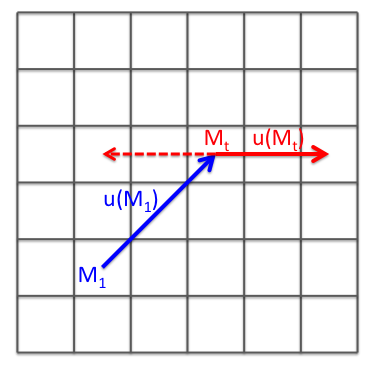
\includegraphics[height=5cm]{figures/fig-invert-trsf.png}
\end{center}
\caption{\label{fig:invert:transformation}$M_t$ is $M_1$ transformed by $T_{t \leftarrow 1}$, i.e. $M_t = M_1 + \mathbf{u}_{t \leftarrow 1}(M_1) $ where $\mathbf{u}_{t \leftarrow 1}(M_1)$ is the blue vector. $T_{t \leftarrow 1}^{-1}$ at $M_t$ should then by defined by the opposite of this blue vector (so that $M_t$ can project on $M_1$). By building the inverse of $T_{t \leftarrow 1}$ with the opposite of the $\mathbf{u}_{t \leftarrow 1}$ vector field, $T_{t \leftarrow 1}^{-1}$ at $M_t$ would be defined by $- \mathbf{u}_{t \leftarrow 1}(M_t)$, i.e. the dashed red vector (and thus not equal to $- \mathbf{u}_{t \leftarrow 1}(M_1)$, the opposite of the blue vector). This can be an acceptable approximation iff $\mathbf{u}_{t \leftarrow 1}(M_t)$ (the red vector) is sufficiently similar to $\mathbf{u}_{t \leftarrow 1}(M_1)$ (the blue vector).}
\end{figure}

$M_t$ is partway on the "line" joining $M_0$ and $M_1$ and at a "distance" $t$   from $M_1$ and $(1-t)$ from $M_0$. 
We have then
\begin{eqnarray*}
M_t =  (1-t) M_0 + t M_1 
& \Leftrightarrow &
 M_0 = \frac{1}{1-t} M_t - \frac{t}{1-t} M_1 \\
& \Leftrightarrow &
 M_0
 = \frac{1}{1-t} M_t - \frac{t}{1-t} T_{1\leftarrow t} M_t \\
& \Leftrightarrow &
 M_0
 = \frac{1}{1-t} M_t - \frac{t}{1-t} 
 \left( M_t + \mathbf{u}_{1 \leftarrow t}(M_t) \right) \\
 & \Leftrightarrow &
 M_0
 =  M_t - \frac{t}{1-t} 
 \mathbf{u}_{1 \leftarrow t}(M_t) \\
\end{eqnarray*}

The transformation $T_{0 \leftarrow t}$ is then represented by the vector field $\left(- \frac{t}{1-t}\mathbf{u}_{1 \leftarrow t}\right)$.

Finally, the image $I_t$ can be interpolated from the resampled $I_0$ and $I_1$ into $I_t$ frame, ie $I_0 \circ T_{0 \leftarrow t}$ and $I_1 \circ T_{1 \leftarrow t}$ with
\begin{displaymath}
I_t = (1-t) \times I_0 \circ T_{0 \leftarrow t}
+ t \times I_1 \circ T_{1 \leftarrow t}
\end{displaymath}